
% This LaTeX was auto-generated from MATLAB code.
% To make changes, update the MATLAB code and republish this document.

\documentclass{article}
\usepackage{graphicx}
\usepackage{color}

\sloppy
\definecolor{lightgray}{gray}{0.5}
\setlength{\parindent}{0pt}

\begin{document}

    
    
\subsection*{Contents}

\begin{itemize}
\setlength{\itemsep}{-1ex}
   \item PROBLEM 1
   \item PART A
   \item PART B
   \item PART C
   \item PART D
   \item PROBLEM 2
   \item SIMULATION TASK 1
\end{itemize}
\begin{verbatim}
clear all;
close all % Clean the workspace
\end{verbatim}


\subsection*{PROBLEM 1}



\subsection*{PART A}

\begin{verbatim}
numerator = [1 2];
denominator = [1 4 8];
H = tf(numerator, denominator); % Define the transfer function
\end{verbatim}


\subsection*{PART B}

\begin{verbatim}
zeros = zero(H); % Find the zeros of the transfer function
poles = pole(H); % Find the poles of the transfer function
pzplot(H); % Plot the plot-zero plot

pause;
\end{verbatim}

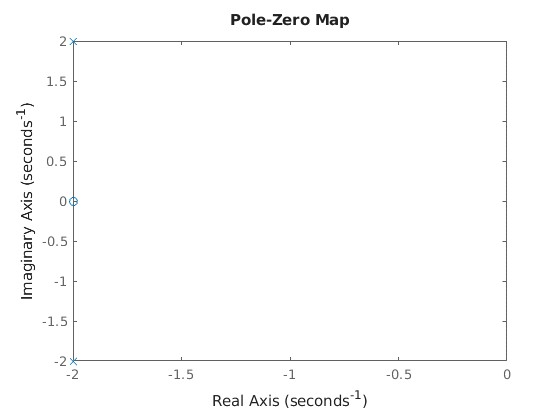
\includegraphics [width=4in]{Figures/CompHW3-1}


\subsection*{PART C}

\begin{verbatim}
impulse(H); % Impulse response plot

pause;
\end{verbatim}

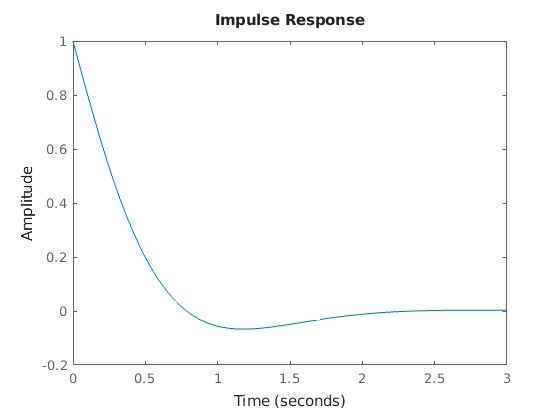
\includegraphics [width=4in]{Figures/CompHW3-2}


\subsection*{PART D}

\begin{verbatim}
t = [0:.01:1]; % Create time array
x = exp(-2 * t); % Create impulse
y = lsim(H, x, t); % Find the response to input
plot(y, t);
xlabel('Response to Given Signal');
ylabel('Magnitude');

clear all;
close all; % Clean the workspace
\end{verbatim}


\subsection*{PROBLEM 2}

\begin{verbatim}
m = 1; % Mass is one kilogram, as given in the problem
k = 1; % k (spring constant) is derived from the requested frequency (1 rad/s)
omega = sqrt(m/k); % Define the requested frequency
v = [2 (1/sqrt(2)) 1/3]; % Define the requested viscosity values
chi = v ./ (2 * sqrt(m*k)); % Define the damping factor

H1 = tf([omega^2], [1 (2 * chi(1) * omega) (omega^2)]);
H2 = tf([omega^2], [1 (2 * chi(2) * omega) (omega^2)]);
H3 = tf([omega^2], [1 (2 * chi(3) * omega) (omega^2)]); % Define the transfer functions
\end{verbatim}


\subsection*{SIMULATION TASK 1}

\begin{verbatim}
hold on; % Plot figures on one plot
pzplot(H1, H2, H3); % Plot the different cases
legend('Case 1', 'Case 2', 'Case 3');

pause;

hold off; % Clear the current figure

t = [0:.1:30]; % Create a 30-second time vector

S1 = step(H1, t);
S2 = step(H2, t);
S3 = step(H3, t); % Compute the three step responses

plot(t, S1, t, S2, t, S3); % Plot the three step responses
xlabel('Frequency');
ylabel('Magnitude');
legend('Case 1', 'Case 2', 'Case 3');

S1_info = stepinfo(H1);
S2_info = stepinfo(H2);
S3_info = stepinfo(H3); % Get the step response info for each system

display('S1 Rise Time, Settling Time, and Overshoot:')
display(S1_info.RiseTime);
display(S1_info.SettlingTime);
display(S1_info.Overshoot);

display('S2 Rise Time, Settling Time, and Overshoot:')
display(S2_info.RiseTime);
display(S2_info.SettlingTime);
display(S2_info.Overshoot);

display('S3 Rise Time, Settling Time, and Overshoot:')
display(S3_info.RiseTime);
display(S3_info.SettlingTime);
display(S3_info.Overshoot);

% We may see that, for larger valus of the dampening factor, the poles
% become close to zero on the imaginary axis and around -1 on the real axis.

% We may observe that a larger rise time corresponds to a larger dampening
% factor. Furthermore, there is more oscillating with smaller dampening
% factor values, which are indicated by the overshoot (with no overshoot
% when chi = 2). We may see that a larger value of the dampening factor
% corresponds to less settling time. The bandwidth is larger with larger
% chi values.

% We may see that a greater dampening leads to lesser magnitude
% fluctuation. Once omega gets to a larger value, chi affects it less.
\end{verbatim}

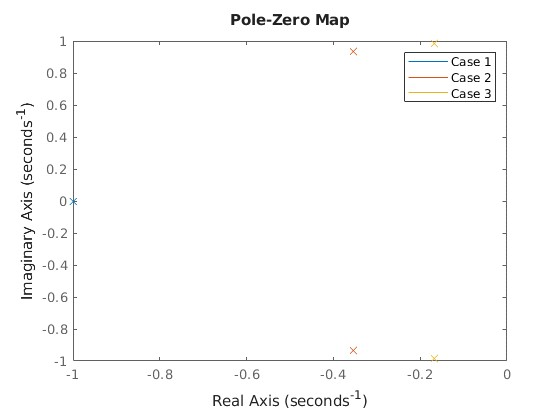
\includegraphics [width=4in]{Figures/CompHW3-3}


        \color{lightgray} \begin{verbatim}S1 Rise Time, Settling Time, and Overshoot:
    3.3579

    5.8339

     0

S2 Rise Time, Settling Time, and Overshoot:
    1.3983

   10.9489

   30.4890

S3 Rise Time, Settling Time, and Overshoot:
    1.1865

   22.9277

   58.3143

\end{verbatim} \color{black}
    
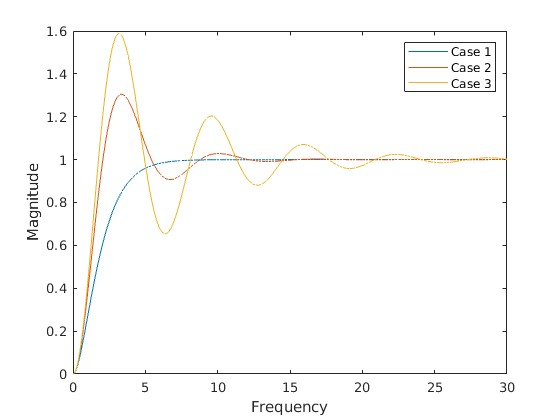
\includegraphics [width=4in]{Figures/CompHW3-4}



\end{document}

